%\documentclass[landscape,pagesize,DIV=14]{scrartcl}
\documentclass[border=2mm]{standalone}

\usepackage[utf8]{inputenc}
\usepackage[T1]{fontenc}

\usepackage{amsmath}

\usepackage{tikz}
\usetikzlibrary{graphs}%,graphdrawing}
\usetikzlibrary{positioning}
\usetikzlibrary{calc}

\newcommand{\code}[1]{\texttt{#1}}
\newcommand{\Owns}[1]{{\color{red}#1}}

\definecolor{mycontour}{HTML}{43709A}
\definecolor{myfill}{HTML}{E2EBF2}
\newlength\separation
\setlength{\separation}{1ex}

\begin{document}

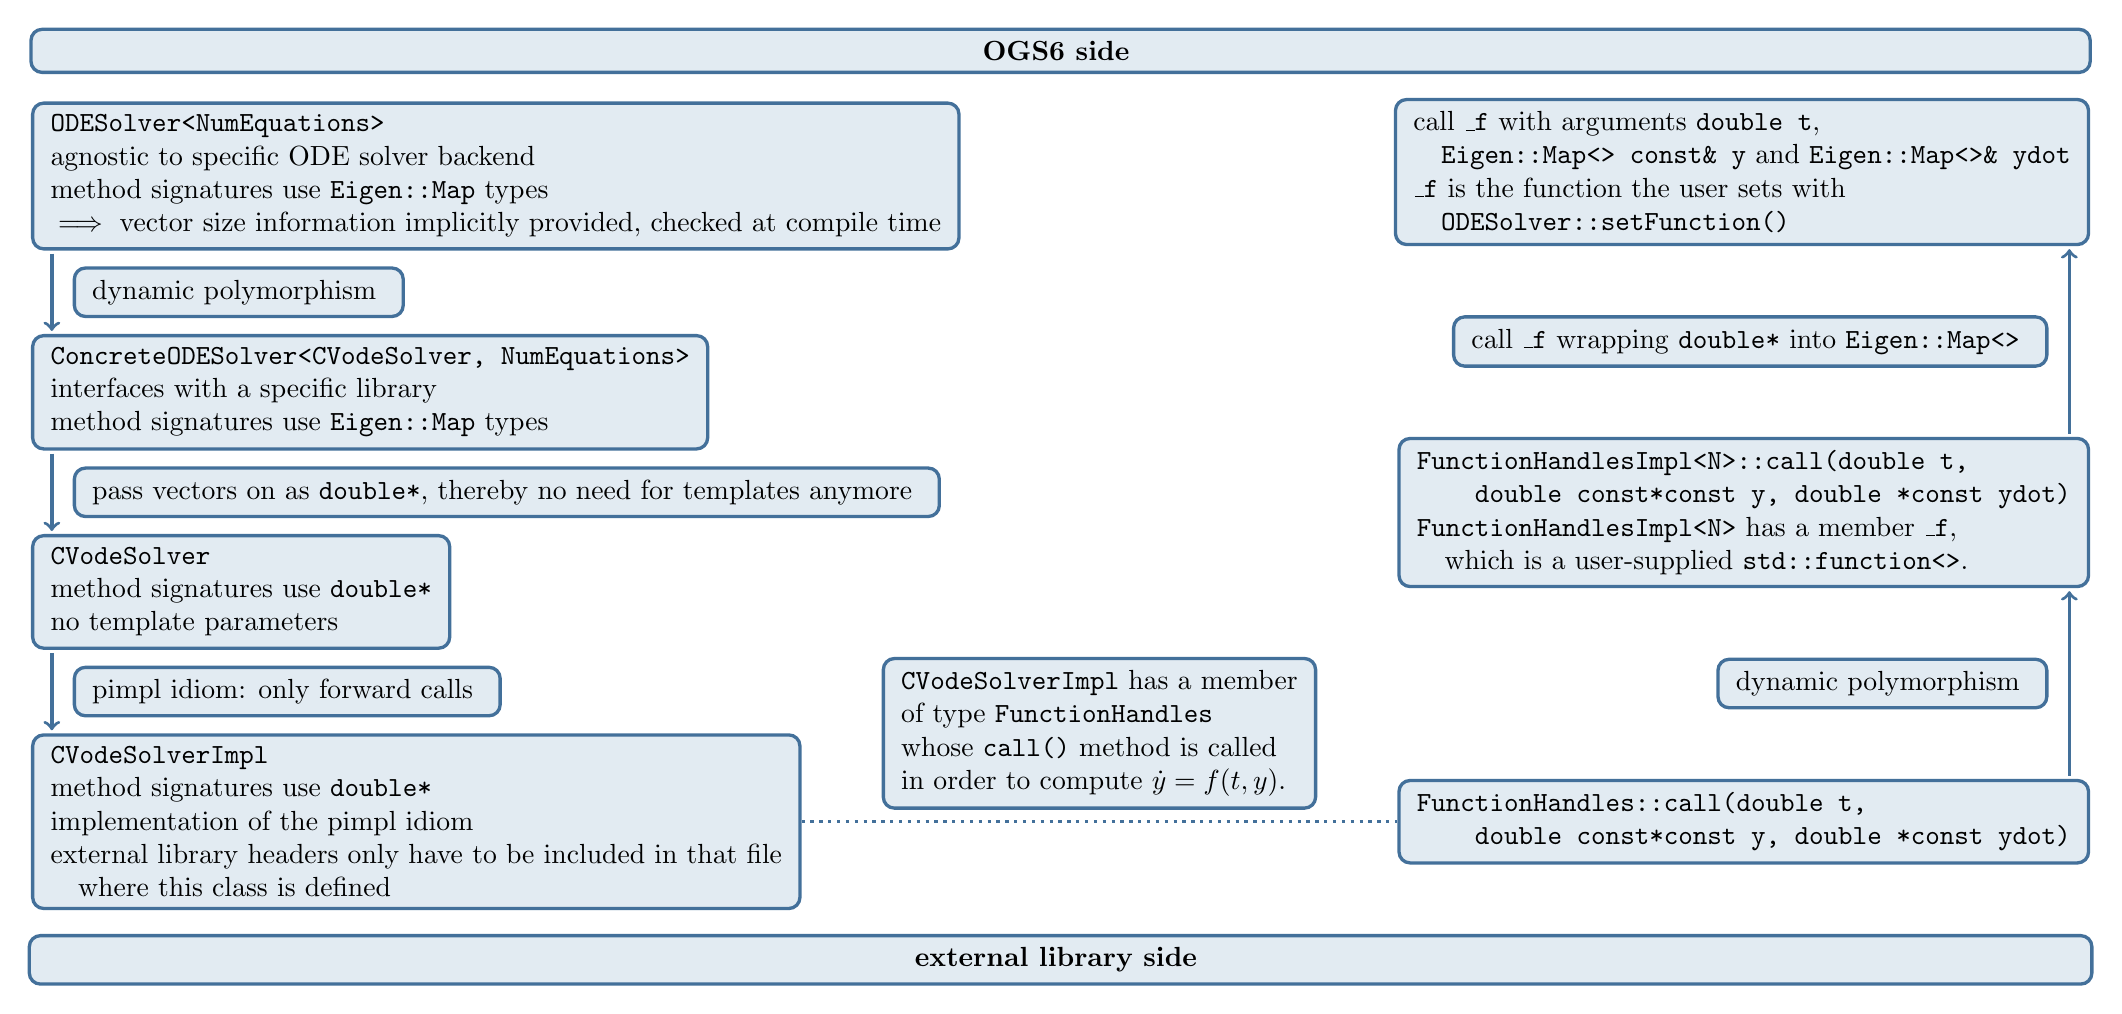
\begin{tikzpicture}[
    very thick,
    align=left, anchor=west,
    %node distance=\separation,
    node distance=7\separation and 0pt,
    color=mycontour,
    text=black,
    every node/.style={
      inner ysep=\separation,
      inner xsep=1.5\separation,
      rectangle,
      rounded corners,
      draw=mycontour,
      fill=myfill
    }
]
  \node (odesolver) at (0, 0) {
    \code{ODESolver<NumEquations>}
    \\ agnostic to specific ODE solver backend
    \\ method signatures use \code{Eigen::Map} types
    \\ $\implies$ vector size information implicitly provided, checked at compile time
  };

  \node (concreteodesolver) [below right=of odesolver.south west] {
    \code{ConcreteODESolver<CVodeSolver, NumEquations>}
    \\ interfaces with a specific library
    \\ method signatures use \code{Eigen::Map} types
  };

  \node (cvodesolver) [below right=of concreteodesolver.south west] {
    \code{CVodeSolver}
    \\ method signatures use \code{double*}
    \\ no template parameters
  };

  \node (cvodesolverimpl) [below right=of cvodesolver.south west] {
    \code{CVodeSolverImpl}
    \\ method signatures use \code{double*}
    \\ implementation of the pimpl idiom
    \\ external library headers only have to be included in that file \\
    \quad where this class is defined
  };

  \draw[->] let \p1=(odesolver.south west), \p2=(concreteodesolver.north west)
  in (\x1+1.75\separation,\y1-.25\separation) --
  node [pos=0.5, right=1.75\separation] {
    dynamic polymorphism
  }
  (\x2+1.75\separation,\y2+.25\separation);

  \draw[->] let \p1=(concreteodesolver.south west), \p2=(cvodesolver.north west)
  in (\x1+1.75\separation,\y1-.25\separation) --
  node [pos=0.5, right=1.75\separation] {
    pass vectors on as \code{double*}, thereby no need for templates anymore
  }
  (\x2+1.75\separation,\y2+.25\separation);

  \draw[->] let \p1=(cvodesolver.south west), \p2=(cvodesolverimpl.north west)
  in (\x1+1.75\separation,\y1-.25\separation) --
  node [pos=0.5, right=1.75\separation] {
    pimpl idiom: only forward calls
  }
  (\x2+1.75\separation,\y2+.25\separation);



  \node (fcthandles) [right=50ex of cvodesolverimpl.east] {
    \code{FunctionHandles::call(double t,}
    \\ \code{~~~~double const*const y, double *const ydot)}
  };

  \node (fcthandlesimpl) [above left=16\separation and 0pt of fcthandles.north east] {
    \code{FunctionHandlesImpl<N>::call(double t,}
    \\ \code{~~~~double const*const y, double *const ydot)}
    \\ \code{FunctionHandlesImpl<N>} has a member \code{\_f},
    \\ \quad which is a user-supplied \code{std::function<>}.
  };

  \node (fct) [above left=16\separation and 0pt of fcthandlesimpl.north east] {
    call \code{\_f} with arguments \code{double t},
    \\ \quad\code{Eigen::Map<> const\& y} and \code{Eigen::Map<>\& ydot}
    \\ \code{\_f} is the function the user sets with
    \\ \quad\code{ODESolver::setFunction()}
  };

  \draw[->] let \p1=(fcthandles.north east), \p2=(fcthandlesimpl.south east)
  in (\x1-1.75\separation,\y1+.25\separation) --
  node [pos=0.5, left=1.75\separation] {
    dynamic polymorphism
  }
  (\x2-1.75\separation,\y2-.25\separation);

  \draw[->] let \p1=(fcthandlesimpl.north east), \p2=(fct.south east)
  in (\x1-1.75\separation,\y1+.25\separation) --
  node [pos=0.5, left=1.75\separation] {
    call \code{\_f} wrapping \code{double*} into \code{Eigen::Map<>}
  }
  (\x2-1.75\separation,\y2-.25\separation);

  \path[-] (cvodesolverimpl.east) edge[dotted]
  node [pos=0.5, above=\separation, solid] {
    \code{CVodeSolverImpl} has a member
    \\ of type \code{FunctionHandles}
    \\ whose \code{call()} method is called
    \\ in order to compute $\dot y = f(t,y)$.
  }
  (fcthandles.west);

  \path let \p1=(current bounding box.west), \p2=(current bounding box.east) in
  node (ogs6)     [above=2ex of current bounding box.north, minimum width=\x2-\x1]
  { \textbf{OGS6 side} };

  \path let \p1=(current bounding box.west), \p2=(current bounding box.east) in
  node (external) [below=2ex of current bounding box.south, minimum width=\x2-\x1]
  { \textbf{external library side} };


\end{tikzpicture}

\end{document}
